\documentclass[12pt, a4paper]{report}
% do not stop on errors
\nonstopmode

\title{Accelerating agent based\\Python models}
\date{\today}
\author{Robert Kruszewski}

\usepackage[usenames,dvipsnames]{xcolor}
%\setlength\parindent{0pt}
\usepackage{tabularx, alltt, amsmath, multirow, graphicx, url, graphics, caption, natbib, listings, fancyhdr,lstlinebgrd,etoolbox,todonotes}

\usepackage[hidelinks]{hyperref}

\lstdefinelanguage[GNU99]{C}[99]{C}
  {morekeywords={asm,__asm__,__extension__,typeof,__typeof__}%
  }%

\lstdefinelanguage[99]{C}%
  {morekeywords={_Bool,_Complex,_Imaginary,auto,break,case,char,%
      const,continue,default,do,double,else,enum,extern,float,for,%
      goto,if,inline,int,long,register,restrict,return,short,signed,%
      sizeof,static,struct,switch,typedef,union,unsigned,void,volatile,%
      while},%
   sensitive,%
   morecomment=[s]{/*}{*/},%
   morecomment=[l]//,%
   morestring=[b]",%
   morestring=[b]',%
   moredelim=*[directive]\#,%
   moredirectives={define,elif,else,endif,error,if,ifdef,ifndef,line,%
      include,pragma,undef,warning}%
  }[keywords,comments,strings,directives]%

\definecolor{lightgray}{rgb}{0.83, 0.83, 0.83}
\definecolor{lightcarminepink}{rgb}{0.9, 0.4, 0.38}

\definecolor{cython-line-1}{rgb}{1,1,0.28}
\definecolor{cython-line-2}{rgb}{1,1,0.91}
\definecolor{cython-line-3}{rgb}{1,1,0.13}
\definecolor{cython-line-4}{rgb}{1,1,0.59}
\definecolor{cython-line-5}{rgb}{1,1,0.83}

\lstset{
  basicstyle=\ttfamily,                   % Code font, Examples: \footnotesize, \ttfamily
  keywordstyle=\color{lightcarminepink},        % Keywords font ('*' = uppercase)
  commentstyle=\color{Gray},              % Comments font
  numbers=left,                           % Line nums position
  numberstyle=\small\color{Gray},                      % Line-numbers fonts
  stepnumber=1,                           % Step between two line-numbers
  numbersep=8pt,                          % How far are line-numbers from code
  backgroundcolor=\color{White}, % Choose background color
  frame=l,
  framerule=1.8pt,                             % A frame around the code
  xleftmargin=0em,
  framexleftmargin=1.7em,
  tabsize=4,                              % Default tab size
  captionpos=t,                           % Caption-position = bottom
  breaklines=true,                        % Automatic line breaking?
  breakatwhitespace=false,                % Automatic breaks only at whitespace?
  showspaces=false,                       % Dont make spaces visible
  showtabs=false,                         % Dont make tabls visible
  columns=fullflexible,                       % Column format
}

\lhead[\rm\thepage]{\fancyplain{}{\sl{\rightmark}}}
\rhead[\fancyplain{}{\sl{\leftmark}}]{\rm\thepage}
\chead{}\lfoot{}\rfoot{}\cfoot{}
\setlength{\headheight}{15pt}
\pagestyle{fancy}

%Our Executive Summary
\renewcommand{\abstractname}{Abstract}
\newcommand{\myparagraph}[1]{\paragraph{#1}\mbox{}\\}

% Better looking chapters headings
\usepackage{titlesec}
\titleformat{\chapter}
  {\normalfont\LARGE\bfseries}{\thechapter}{1em}{}
\titlespacing*{\chapter}{0pt}{3.5ex plus 1ex minus .2ex}{2.3ex plus .2ex}

\begin{document}

\begin{titlepage}

\newcommand{\HRule}{\rule{\linewidth}{0.5mm}} % Defines a new command for the horizontal lines, change thickness here

\center % Center everything on the page

%----------------------------------------------------------------------------------------
%   HEADING SECTIONS
%----------------------------------------------------------------------------------------

\textsc{\large Imperial College London}\\[1.5cm] % Name of your university/college
\textsc{\large Department of Computing}\\[0.5cm] % Major heading such as course name
\textsc{\large}\\[0.5cm] % Minor heading such as course title

%----------------------------------------------------------------------------------------
%   TITLE SECTION
%----------------------------------------------------------------------------------------

\HRule \\[0.4cm]
{ \huge \bfseries Accelerating agent based\\\vspace{0.4cm}Python models}\\[0.4cm] % Title of your document
\HRule \\[1.5cm]

%----------------------------------------------------------------------------------------
%   AUTHOR SECTION
%----------------------------------------------------------------------------------------

\begin{minipage}{0.4\textwidth}
\begin{flushleft} \large
\emph{Author:}\\
Robert Kruszewski\\
\end{flushleft}
\end{minipage}
~
\begin{minipage}{0.4\textwidth}
\begin{flushright} \large
\emph{Supervisors:} \\
Dr. Anthony \textsc{Field} \\% Supervisor's Name
Dr. Michael \textsc{Lange} \\% Supervisor's Name
%Michael \textsc{Hadjiyiannis}
\end{flushright}
\end{minipage}\\[5cm]

% If you don't want a supervisor, uncomment the two lines below and remove the section above
%\Large \emph{Author:}\\
%John \textsc{Smith}\\[3cm] % Your name

%----------------------------------------------------------------------------------------
%   DATE SECTION
%----------------------------------------------------------------------------------------

{\large \today}\\[3cm] % Date, change the \today to a set date if you want to be precise

%----------------------------------------------------------------------------------------
%   LOGO SECTION
%----------------------------------------------------------------------------------------

%\includegraphics{Logo}\\[1cm] % Include a department/university logo - this will require the graphicx package

%----------------------------------------------------------------------------------------

\vfill % Fill the rest of the page with white space
\end{titlepage}
%% Ending of title page


\begin{abstract}
\todo{ABSTRACT}
\end{abstract}

\renewcommand{\abstractname}{Acknowledgements}
\begin{abstract}
\todo{ACKNOWLEDGEMENTS}
\end{abstract}

\pagenumbering{roman}
\tableofcontents
\listoffigures
\lstlistoflistings
\todototoc
\listoftodos

\chapter{Introduction}\label{ch:intro}
% Reset page numbers
\pagenumbering{arabic}

\todo{INTRODUCTION}
\section{Motivation}\label{sec:intro-motiv}
\section{Objectives}\label{sec:intro-obj}
\section{Contributions}\label{sec:intro-contrib}
% We want to use Python due to widespread use in research field.
% The problem - Python (CPython) isn't truly multithreaded
%     CPython (interpreter in use) has GIL
%         other implementations would be difficult to embed in C/Fortran code base

% \section{Contributions}\label{sec:contributons}
% \begin{itemize}
%     \item Familiar syntax
%     \item Same performance as pure C
%     \item Allows for multithreading and can be deployed in real life applications
% \end{itemize}

\chapter{Background}\label{ch:bkg}

\section{Modeling Plankton Ecosystems}\label{sec:model-plankton-eco}

With plankton contributing about 70\% of oxygen production and
constituting most of biological production on the planet it has
become important to understand systems in which it develops and
grows. Due to its abundance it has a large impact on earth's
atmosphere, particularly regulation of carbon dioxide amounts.
Understanding beneficial and harmful effects of human's influence
on the oceans is one of the most challenging open scientific
problems. Being the fundamental element of every marine ecosystem
understanding plankton development is crucial.

Marine ecology can be understood by observations. It involves
taking measurements in specified region and computing statistical
properties in question. This process is limited with its scale
and require understanding of the context in which the measurements
re taken. On the other hand mathematical simulation involve creating
abstract representation of the environment and objects in it and
allow the underlying principles develop the ecosystem through time.
Despite the fact that our knowledge of marine ecosystems is limited
we do have good understanding of several basic processes. Therefore
methodologies that allow specifying behaviour in terms of primitive
biological equations which allow for demographic properties to emerge
from simulation are likely to be more accurate. Thus any number of
scenarios can be created and What-if? predictions can be carried out.
Naturally the accuracy of those predictions depends on correctness
of the simulation itself.

The model needs to simulate the whole ecosystem: the chemical environment,
the underlying physics principles and interaction between agents themselves
as well as environment. Those requirements lead very quickly to complex systems
that need a lot of computational power. Furthermore the simulation framework
should be general enough to accommodate changing environment; different chemical composition,
varied species and changes in physical conditions.

What remains constant between different ecosystems is the method which governs interactions
between elements and how the system develops over time irrespective of the environment
under consideration. The procedure which underpins the model is called a Metamodel\ref{sec:meta}
and is a design decision when creating simulation software.

\section{Metamodel}\label{sec:meta}
Plankton ecosystems can be classified according to the metamodels which govern
the way the plankton is aggregated. Throughout the years four metamodels have
been developed, i.e. box, field, Lagrangian ensemble (LE) and individual. They
are of increasing computational complexity and apart from LE metamodel present
completely different approach to the problem. The box metamodel is on one end
of the spectrum where the organisms are represented by average value of
properties in certain volumetric space. The individual model, however,
models every organism as a separate object thus allowing to describe the system
in terms of primitive biological equations.

\subsection{Field Metamodel}\label{para:field-meta}
The field metamodel uses spatial fields to describe the plankton population.
It considers the properties that the system is composed of and for each
of them constructs continuous field over the space in question. Such
treatment does not allow to model individual organisms but instead
focuses on the demographic properties of the population, i.e. what is
density of certain value at given point instead of allowing for free
interaction of organisms with the environment and each other.

Since there is no need to model each organism individually but only
each property using this metamodel lowers computational complexity
but forces modeling at higher level of the system. That is the
properties of the system and their changes in time have to be studied
and behaviour has to be extracted. While in nature the behaviour of
individual organisms lends itself to emergence of patterns in changes
of system properties.

\myparagraph{Spatial Field}\label{par:field}
Spatial Field $F$ is a function of n dimensional spatial variables.
We distinguish two types of fields: scalar, where the function $F$
takes scalar values, e.g. concentration of chemical element at certain
point $(x,y)$ and vector, which takes on vector values, like
velocity of wind at location $(x,y,z)$.

Usually the measurements will be obtained as discrete set of points.
Therefore the function $F$ is obtained from finite set of
measurements $$F(x_1,y_1),\ldots,F(x_N,y_N)$$ performed at $N$ discrete
points $(x_i,y_i)$

\subsection{Individual Metamodel}\label{subsec:agent-meta}
The individual metamodel is the extreme end of the modeling spectrum.
The aim is to represent each organism in the simulation as an object
and let those interact with environment and each other. Such models
quickly become complex with due to the size of the simulated problem
and require large amount of computational power. Their emergence
was only possible due to rapidly rising computer power.

The benefit of individual based metamodels over field and box metamodels
is the ability to use primitive biological equations to represent
elements of simulation. Those equations can be obtained by observation
of individuals of desired species and does not involve analyzing
large population. As a result the model will represent the nature
more accurately and gives a possibility of accurate results and
therefore better predictions. As has been mentioned the downside
is the computational complexity.

\subsection{Lagrangian Ensemble Metamodel}\label{subsec:le-meta}
Combination of field and individual based metamodel allows for trade-off
between accuracy of the model and complexity. The Lagrangian Ensemble
metamodel uses biologically-lagrangian integration to follow the life
history of each plankter, and ensemble statistics to compute the bulk proper-
ties of whole populations. In such it behaves like individual based model
when considering single organism but at the same time uses spatial fields
to describe the properties of the population.

The Lagrangian Ensemble metamodel results in a compromise between field
and individual based approaches. As a way to achieve the flexibility
each agent in the simulation represents number of identical individuals.
The sub-population of an agent is dynamic and governed by particle
management rules. In the extreme Lagrangian Ensemble metamodel can
approximate individual based metamodel, i.e. when sub-population size is
set to 1. On the other extreme it can be used to represent field metamodel
by creating only one subpopulation. With the ability to adjust
sub-population size of agents the LE metamodel allows us to address
computational performance while limiting demographic noise.

\section{Virtual Ecology Workbench (VEW)}\label{sec:vew}
The Virtual Ecology Workbench (VEW) (shown in figure \ref{fig:VEW})
is a software suite that provides tools to make plankton ecosystem
simulations in a mid-ocean mesocosm easy. It is aimed at biological
oceanographers, thus doesn't require programming knowledge. It uses
Lagrangian Ensemble metamodel to govern the simulation. In this
metamodel the emergent demographic properties are derived from
individual based agents which in turn are described
using primitive biological equations. Each simulation created
by VEW is globally stable, adjusts to attractor that is independent
of initial condition \cite{Woods2005}. Therefore such simulations
are useful for What-if? Prediction.

\begin{figure}[ht!]
  \begin{center}
    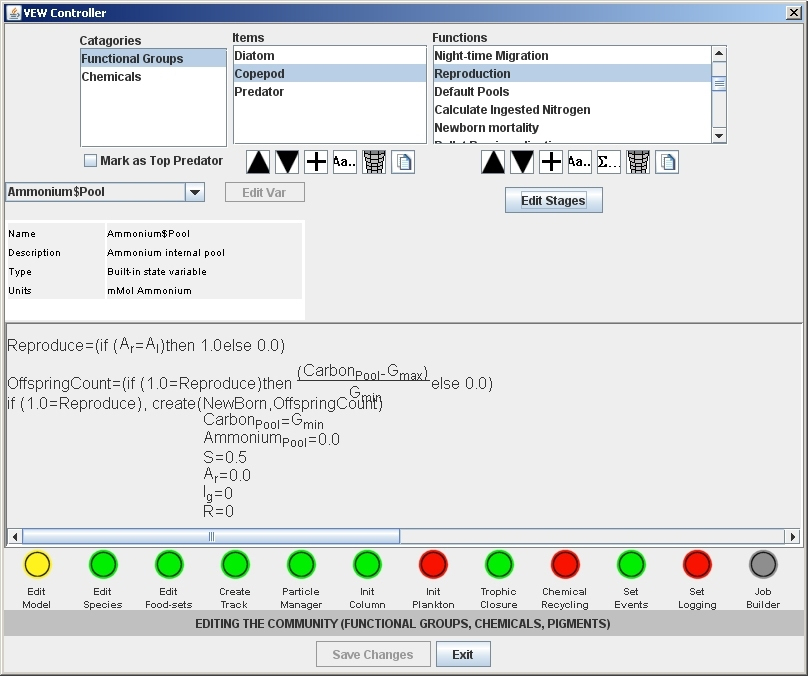
\includegraphics[width=0.7\textwidth,natwidth=808,natheight=676]{images/vew2007-10.jpg}
    \caption{Look at Virtual Ecology Workbench GUI of equation editor}
    \label{fig:VEW}
  \end{center}
\end{figure}

Virtual Ecology Workbench enables users to create simulation using
phenotypic equations in form familiar to them. It automatically
generates necessary code to represent environment and species
specified by user. The Lagrangian Ensemble metamodel
provides good trade-off of computational complexity and accuracy.
The metamodel computes emergent properties, the demography
of species population and biofeedback between agents and environment.
The simulation describes life history of every individual plankter
in the ecosystem to make it possible. Each agent in the simulation
behaves like a population of multiple identical plankters. Each
plankter in the ecosystem is contained in one of those agents.
Simulation created by VEW employ splitting and merging techniques
to ensure that that population is adequately represented and
that sampling is accurate where each agent can be subdivided into
multiple or two agents can be merged together. Therefore the
total number of agents can always stay within boundaries
defined by the user.

\subsection{Environment}\label{para:1d-phys}
\begin{figure}[ht!]
  \begin{center}
    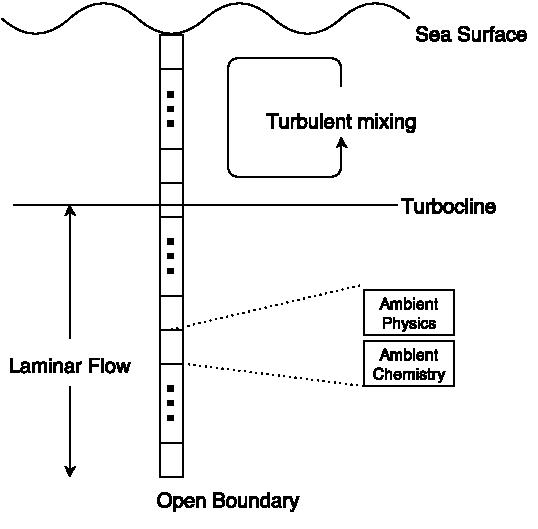
\includegraphics[width=0.6\textwidth,natwidth=473,natheight=466]{images/env-diagram.pdf}
    \caption{Physical environment in which VEW carries out the simulation}
    \label{fig:env}
  \end{center}
\end{figure}

Figure \ref{fig:env} illustrates the environment that is employed by VEW
to carry out its simulation. The physical environment as defined by Woods \cite{Woods2005}
is a one-dimensional water column for us in open ocean where water depth exceeds 1km.
The vertical axis extends from the sea surface to depth of, typically, 0.5km.
VEW allows for the column to drift with ocean currents or be hoisted in place.
Solar and infra-red radiation, sensible and latent heat, water vapour
and other gases pass through the upper boundary while the lower is open
and allows detritus to sink through to the deeper parts of the ocean.
The physical model makes an assumption that even though the
water can flow freely through side walls of the environment it produces
zero flux divergence in every ecosystem property at all depths.

There are two reasons why approximation through one-dimensional model is
acceptable and will produce good results. First of all, the plankton being
modeled lives mostly in seasonal boundary layer of the ocean which has structure
controlled mostly by vertical fluxes. Secondly, the horizontal correlation
scale of the environment variables is typically two orders of magnitude greater
than the vertical scale. Planktons cannot usefully change their ambient environment
by swimming horizontally. However, many species of plankton do change their
ambient environment by swimming horizontally. This one-dimensional model is a very
good first approximation. It has to be noted though that the principal source
of errors arises from the neglect of mesoscale turbulence which is mostly correlated
in horizontal scale. Simulation of plankton ecosystems with mesoscale turbulence
requires three dimensional version of LE metamodel. In work by Lange \cite{FluidityVEW}
the author shows how to integrate VEW generated models into general computational
fluid dynamics framework and demonstrates that the resulting system adjusts to
similar attractors as one-dimensional version.

\subsection{Functional Groups}\label{subsec:fg}

At the core of Lagrangian Ensemble modeling there are functional groups (FG).
Functional groups are the highest level grouping in marine biodiversity
parameter space. It defines set of variables that represent agent's internal
biochemical state. Furthermore it is used to define the set of phenotypic
equations that govern physiology and behaviour which are used to advance
agent to next time step.

\begin{figure}[ht!]
  \centering
  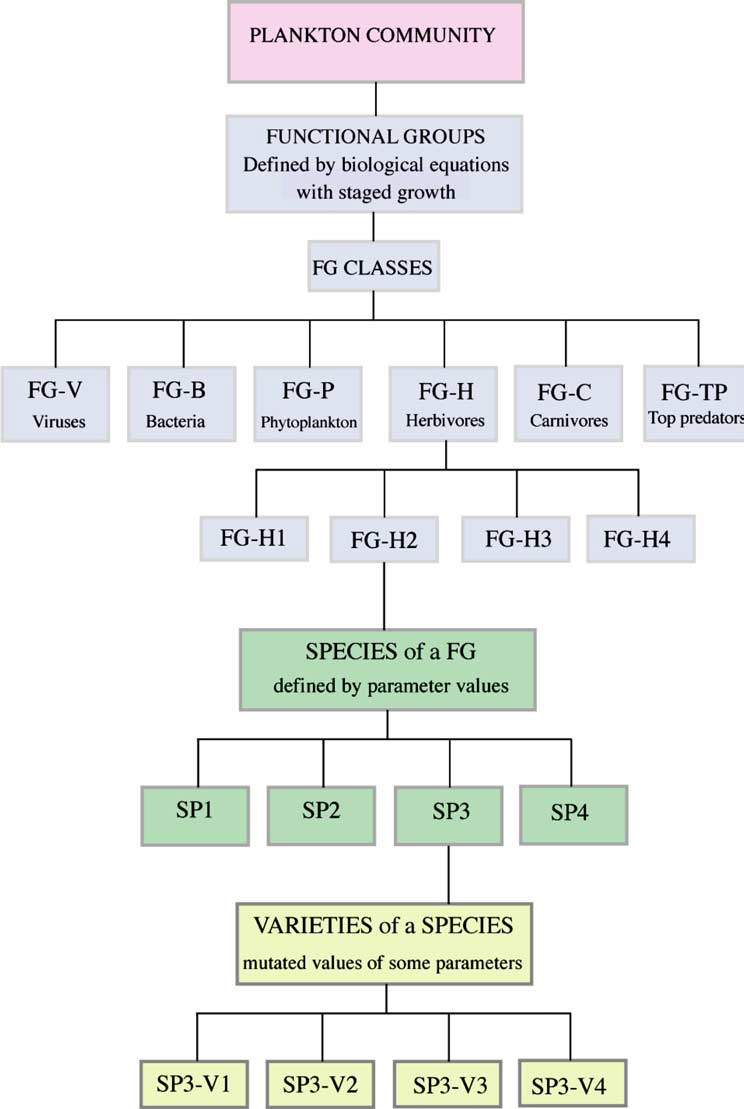
\includegraphics[width=0.7\textwidth,natwidth=744,natheight=1109]{images/fg.jpg}
  \caption{Plankton community according to Woods \cite{Woods2005}
    with functional groups, species and varieties}
  \label{fig:fg}
\end{figure}

Figure \ref{fig:fg} shows grouping hierarchy of ecosystem modeling
objects. The plankton community in simulation consists of multiple functional
groups. Each of communities may be later subdivided into species. In case of
LE modeling species define parameter set for enclosing functional group set of
equations. Through parameter mutation we can achieve multiple varieties of
species. Going further down each species can be subdivided into traits.
Traits allow to factor in ecological adaptation in resource competition models.
As such traits are a way to incorporate evolution into ecosystem models
which is a current trend in modeling \cite{Clark20113823}.

The major difference in Lagrangian Ensemble model as proposed by Woods
\cite{Woods2005} is the ability to capture life-cycle of individual. This
feature is impossible to emulate in population-based approaches. As a
consequence each agent can have particular stage associated with it. Agent's
stage defines physiological processes currently active in subpopulation hence,
the phenotypic equations that are being used at particular timestep. The LE
allows for incorporation of growth, dormant stages and over-wintering as
seen in nature. The metamodel acknowledges the fact that physiological
behaviours of individuals may change over time and thus should be represented
in the model. Different growth stages constitute important source of intra-population
variability in ecosystem modeling.

\subsection{Model Specification - Planktonica}\label{subsec:planktonica}
The way in which model is specified in Virtual Ecology Workbench is through
Planktonica \cite{Planktonica}. Planktonica is a modelling language for
designing plankton. Arbitrary chemicals, with different action spectra to
represent pigmentation, can be used. Planktonica allows for encapsulation of
metamodel which describes basic rules in which simulation is carried out
like the definition of particle, the way the may interact and definition
of environment.

Planktonica creates the simulation code from the high level description
provided by the user. Thus it does not require programming knowledge.
The descriptions provided are transformed to an XML model which is
further enriched by later stages of VEW pipeline. Finally Planktonica
itself generates the code required to run the simulation for specified
model. Figure~\ref{fig:planktonica} Illustrates how the parts of the system
communicate together.

\begin{figure}[ht!]
  \centering
  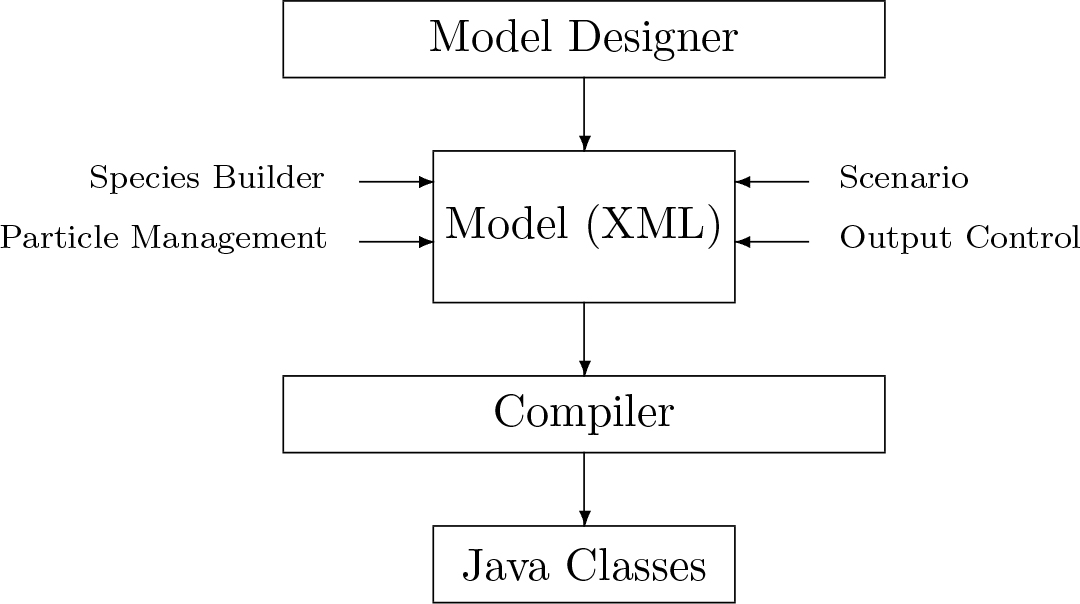
\includegraphics[width=0.7\textwidth,natwidth=1080,natheight=604]{images/planktonica.jpg}
  \caption{Schematic working of Planktonica taken from Hinsley \cite{Planktonica}}
  \label{fig:planktonica}
\end{figure}

\subsection{Agents}\label{subsec:agents}
Lagrangian Ensemble metamodel has the ability to represent
multiple organism from same subpopulation into one agent.
Therefore plankton in the simulation can be described in
terms of primitive biological equations which are
observable in laboratory experiments. Instead of defining
each elements behaviour separately the LE metamodel uses
functional groups, species and stages to define set of
variables that govern its state and transitions.
Due to independence of agent updates from state all of the
biochemical processes can be defined once for any species
in particular stage. This is to the contrary to field models
where each property changes differently depending on a location
on a fixed mesh\cite{Woods200543}. Furthermore agents are able to
nondeterministically change their internal biological
state via stage transitions. In order to manage
those extra care has to be taken in particle management.

\subsection{Physics - Particle Management}\label{subsec:physics}
Due to individual based nature agent based model require a sampling
strategy to represent large number of plankters per cubic metre in the
ocean while keeping the problem computational feasible. This is achieved
in Lagrangian Ensemble metamodel via number-based up-scaling mechanism,
i.e. single agent represents multiple identical individuals. In order
to be able to compute demography of the population realistically
every individual has to occur in one of the agents present in the
environment. Due to the fact that number of individuals may change
significantly during particular time step. Therefore agent accounting
method is necessary to keep the number of agents during simulation
in desired range.

Restriction on number of agents are enforced by Particle Management.
The manager provides the trade-off between accuracy and speed of the
simulation. In order to enforce bounds specified by the user
the agent population is re-sampled using a continuous split/combine
algorithm. The number of agents is increased in a given region
by splitting the largest of agents in the set evenly until
the minimum threshold value is surpassed. Converse happens when
merging. The smallest agent in region are merged in pairs of two
and resulting agent has the weighted average of variables from source
set.

\begin{figure}[ht!]
  \begin{center}
    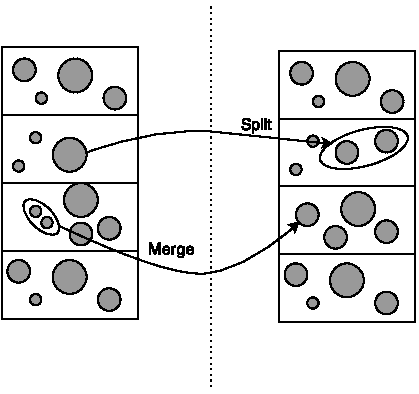
\includegraphics[width=0.4\textwidth,natwidth=366,natheight=342]{images/Split_merge.pdf}
    \caption{Example of Split/Merge in action}
    \label{fig:split-merge}
  \end{center}
\end{figure}

This method is illustrated in Figure \ref{fig:split-merge},
where a target density of four agents per level is requested.

\section{Fluidity}\label{sec:fluidity}
The biggest disadvantage of models generated by VEW is the 1D environment.
It does not allow for horizontal movement and according to authors
``serves as a good first approximation'' \cite{Woods2005}. It is still an approximation.

In work done by Lange \cite{FluidityVEW} Fluidity, general-purpose
computational fluid dynamics software, has been adapted to incorporate
ocean modelling. Fluidity \cite{Piggot2008,fluidity} is capable of
solving Navier-Stokes equations and accompanying field equations on
arbitrary unstructured finite element meshes. The computation is
parallelised using MPI and uses adaptive remeshing to optimize the
underlying mesh structure at runtime. Therefore achieving computational
efficiency and focus on regions of interests. The resulting Fluidity-ICOM
provides ocean model capable of sub-grid scale parametrization to model
turbulent mixing as well as embedding of plankton biochemistry.

Fluidity is highly configurable via graphical user interface tool Diamond
which comprises larger scheme-driven description library Spud\cite{ham2009spud}.
Using the tool users are able to define properties to be computed during the simulation.
Fluidity has three types of fields \cite{fluidity}:

\begin{itemize}
  \item Prognostic fields are computed through solving partial different equations.
    User can specify discretisation used during solve phase as well as initial and boundary
    conditions via Diamond.
  \item Diagnostic fields are computed from other fields without solving a
    partial differential equation.
  \item Prescribed fields are defined by external sources. They can encapsulate a constant
    or a user defined function which can, i.e. be used to derive environment condition
\end{itemize}

\subsection{3D Particle Management}\label{subsec:3d-pm}
The key motivation for using Fluidity to model the physical environment
is the ability to introduce individual based plankton simulations in three
dimensional setting. With 3D meshes the impact of mesoscale turbulence,
only possible with turbulent ocean dynamics, on plankton simulations
can be investigated. In order to ensure correctness of the simulation
the interplay between ocean dynamics and ecological factors of marine
plankton ecosystem the ocean model has to be capable of resolving
turbulent flows at varying scales and resolutions.

VEW based models do not resolve turbulent nutrient dissipation within
surface mixed layer but enforces it. Fluidity has inherently different
model where it solves advection-diffusion equation with numerical eddy
diffusivity to achieve turbulent nutrient dissipation.
VEW generated simulation rely heavily on accurate convection based
cycle of mixed layer deepening. The key challenge is to integrate
mixed layer depth model used in VEW and Fluidity's advection-diffusion
equations. In order to achieve the desired effect K-profile parametrisation
is used alongside VEW's MLD model.

\myparagraph{Adaptive Remeshing}\label{para:remesh}
What makes Fluidity attractive for large scale simulations is its ability
to dynamically adapt the underlying mesh at runtime. The process minimises
discretisation errors and focuses resolution on regions of particular interest.
The adaptive mesh refinement uses anisotropic metric tensor field which
describes desired geometric properties necessary to minimise interpolation error.
The metric tensor can be formed from multiple fields and is computed using
Hessian of the fields under consideration. Therefore Fluidity's adaptive
mesh will have higher resolution in areas of steep gradients and coarser
in regions with smooth transitions.
From point of view of ocean modelling the ratio between horizontal
and vertical dimensions should be high. Particularly is mesoscale processes
are to be resolved. Fluidity has the ability to decouple vertical
and horizontal adaptation steps resulting in columnar mesh where elements
are aligned vertically and extruded from underlying horizontal two-dimensional mesh.
The vertical resolution is adapted independently of horizontal and allows
for linking between all columns to form a layered mesh.

\subsection{Model Specification - Python}\label{subsec:model-spec-py}

\begin{figure}[ht!]
  \begin{center}
    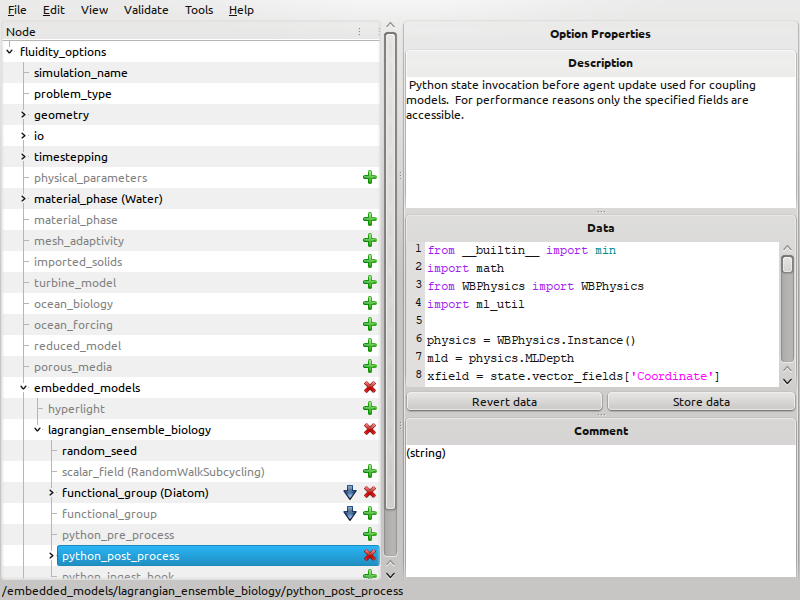
\includegraphics[width=0.7\textwidth,natwidth=800,natheight=600]{images/diamond.png}
    \caption{Diamond - Fluidity's configuration creator}
    \label{fig:diamond}
  \end{center}
\end{figure}

Python is used throughout Fluidity-ICOM implementation to provide flexible
interface which serves as a further customisation to configuration options.
The provided Python code is used to prescribe and manipulate field data.
Fluidity employs CPython via it's C-API to allow on the fly computation
of user provided options.

Diamond, show in Figure \ref{fig:diamond} is used in Fluidity to provide easy way to modify large
configuration files. Python code can be conveniently embedded via its
interface.

The embedded interpreter is used two fold
\begin{itemize}
  \item Space and time-varying field data - Space and time-varying field
data may be entered as a Python function to define prescribed fields
or enter the initial condition of a prognostic field.
  \item Internal State - Fluidity provides access to internal state
  and field data via Python interface. Through this interface
  the user can define own diagnostic algorithms where diagnostic
  field values are set by user defined Python functions. The interface
  may also be used to define ecology models by specifying relevant
  source and absorption terms of the prognostic fields representing
  the ecosystem elements.
\end{itemize}

\section{LERM}\label{sec:lerm}
Throughout this thesis the model employed is based on
Lagrangian Ensemble Recruitment Model (LERM) as first designed
by Sinerchia et al. \cite{FisheriesRecruitment}. LERM is a
fisheries recruitment model that uses four trophic levels to
model the effects of predation and competition on squid recruitment.

\subsection{Simple LERM}\label{subsec:lerm-simp}
While the original model provides realistic example in order
to focus on performance aspects of simulation as simplified version
is used. Thus only Diatoms, plant-based plankters, are present
as agents. Top level predators as well as Copepods (animal-based plankton)
are ignored in this version of the model. There is no predation
between agents, hence there is no need to simulate ingestion.
While those restrictions focus biological environment we will also
disregard bio-optical feedback and read physical environment
information: temperature, visible irradiance, level of turbocline
layer and depth of water column, from files generated by
full Java based VEW simulation.

\subsection{Simple LERM in Fluidity}\label{subsec:lerm-simp-fluid}
\todo{explain difference between simple LERM and 3D Fluidity Model}


\section{Parallelisation}\label{sec:para}

\subsection{OpenMPI}\label{subsec:openmpi}
Message Passing Interface is a way of distributing computation
amongst several machines via network connection. Each of the
machines (nodes) in the system is able to issue and receive
messages which are a way to synchronize and distribute data.
OpenMPI \cite{gabriel04:_open_mpi} is a result of merger of several MPI libraries, like
LAM/MPI, LA-MPI, and FT-MPI. It aims to standardise the implementation
and improve interoperability. Thus reducing the burden on
end users and increasing adoption. It provides production-quality
MPI-2 implementation. Currently OpenMPI is de-facto the MPI
library. Apart from being a quality MPI implementation is to
facilitate third-party research and creation of independent
add-ons.

\subsection{OpenMP}\label{subsec:openmp}
While OpenMPI focuses on distributing workload amongst different
machines OpenMP \cite{OpenMP4.0} is used to distribute tasks in one machine amongst
several cores. Due to it's memory oriented nature there's a significant
penalty incurred when operating across different cache domains.
OpenMP aims to provide compiler directives, library routines, and environment variables
for shared-memory parallelism in C, C++ and Fortran programs.

In contrast to other multithreading approaches OpenMP provides high
abstraction level thus enabling portability. The portability of OpenMP directives
is ensured by runtime library which is platform dependent part of implementation.
The directives it introduces focus on single program multiple data
(SPMD) constructs, tasks, worksharing and synchronisation.
Furthermore the library provides means of sharing and privatizing
data across threads.

OpenMP only covers user-directed parallelization, where programmer explicitly
states actions which are to be taken by compiler to make program parallel at runtime
Any implementation is not required to check for data dependencies, data conflicts,
race conditions, or deadlocks which may occur in multithread programs.
The specification does not cover compiler-generated automatic parallelization and
directives to the compiler to assist such parallelization.

Since OpenMP is tightly integrated with the compiler it is non-trivial to
understand types of transformation that are performed to make program parallel.
Listing \ref{list:openmp-dir} and \ref{list:openmp-run} shows one of the transformation that is performed.

\begin{lstlisting}[
  caption=Code with OpenMP directives,
  label=list:openmp-dir,
  language=c
]
#include <omp.h>
void main() {
  #pragma omp parallel
  {
    int ID = omp_get_thread_num();
    printf(“Hello world(%d)”, ID);
  }
}
\end{lstlisting}

\begin{lstlisting}[
  caption=Code from \ref{list:openmp-dir} with substituted runtime library calls,
  label=list:openmp-run,
  language=c
]
void __ompregion_main1(...) {
  int ID = ompc_get_thread_num();
  printf(“Hello world(%d)”,ID);
} /* end of ompregion_main1*/

void main() {
  ...
  __ompc_fork(&__ompregion_main1,...);
  ...
}
\end{lstlisting}

\subsection{Isoefficiency}\label{subsec:isoeff}
Isoefficiency is a measure of how in relation to growth in number of parallel execution units the working set has to grow in order to maintain same efficiency of the system. In general with growing working set size given constant number of processors the efficiency increases while the inverse happens when working set size is constant and number of parallel execution units increases.
\begin{equation}\label{eq:isoeff} W = \dfrac{E}{1-E}T_o(W,p) \end{equation}
\ref{eq:isoeff} describes relation between working set size and efficiency for parallel system as defined in \cite{grama2003introduction}.
For any scalable system efficiency can be maintained at a fixed value if the ratio \[\dfrac{T_o}{W}\] is kept at a constant value.
Let \[K = \dfrac{E}{1-E}\] be a constant depending on the efficiency to be maintained. The we have
\begin{equation}\label{eq:isoconst} W = KT_o(W,p) \end{equation} Knowing properties for a particular system we can obtain value of W
as a function of p which dictates the rate at which working set size has to grow in order to maintain fixed efficiency.

\subsection{Python Multithreading}\label{subsec:mult-py}
Python as a programming language dates back to beginning of 90s. Since that
time it has grown to be one of the most widely used general purpose scripting
languages. Due to its high abstraction level it allows expressing concepts in
few lines of code. Furthermore it provides large standard library.

Python is a truly multithreaded language. Each of the threads that are spawned
by interpreter are first class operating system threads. As such Python gives
ability to write applications running on large machines. There's a caveat, namely
the Global Interpreter Lock (GIL). Due to GIL besides threading concurrency model
Python provides process level concurrency. Since each process has its own address
space and memory they do not interfere with each other and can run in parallel.
Due to inter process communication there is a significant overhead incurred
when passing values around between processes. In order to mitigate the drawbacks
of memory passing Python aims to provide non blocking interfaces for I/O and
networking operations which effectively make explicit threading redundant. However,
Python does not have a good solution for threading CPU intensive programs. There are
numerous extensions, most prominent of which are NumPy and SciPy. Those libraries aim to provide
true parallelism for CPU intensive operations. However, they achieve this effect
not in pure Python but by delegating the computation to external C or Fortran modules
which can run unaffected by GIL.

It has to be noted that Python as a language has multiple implementations. Most
widely used are CPython (reference implementation), PyPy (CPython compatible implementation
with JIT capabilities), IronPython (Python implementation in C\#)
and Jython (JVM based implementation). The GIL problem only applies to CPython
and implementations that are compatible with it. Given the fact that other
versions don't have widespread adoption Python is often exclusively associated
with CPython. Given the fact that majority of Python modules are written to conform with
CPython API any implementation without CPython compatibility stands little chance
of widespread adoption and success.

\subsection{Global Interpreter Lock (GIL)}\label{subsec:GIL}
The Python reference implementation (CPython) has been written with Global
Interpreter Lock. What GIL does is to ensure that only one thread at a time
modifies the internal memory of interpreter. This in turn is necessary
due to CPython memory model. By using reference counting for garbage collection
CPython removes burden of explicit memory management, however, for the
scheme to work the reference counts have to be accurate. Therefore whenever
an object in Python is created and modified the thread has to acquire an
exclusive lock for memory modification. As a result of GIL regardless
of number of threads if the application wants to interpret Python code
it will use only one thread. This behaviour is a bottleneck for CPU
intensive applications rendering them exclusively single threaded.

\myparagraph{Removing GIL}\label{para:remove-gil}
With shift from faster processors to more cores per processor in CPU
design the GIL had become a central issue to threading Python code.
First proposal to remove GIL from Python occurred in 1999 when Greg Stein
replaced GIL in Python 1.5 with fine-grained locks \cite{Guido:GIL}. However, the resulting
code was almost two times slower than version with global lock,
moreover there was no clear gain from threading the interpreter due
to lock contention being a bottleneck. As a result the changes have
disappeared over time. The need to remove GIL lessened over time
with development of modules which operate in pure C or Fortran code
and therefore can be treaded. In case of I/O and networking the
problem is mitigated with asynchronous calls. GIL remains issue
only for CPU intensive tasks.

There are downsides to removing GIL though. Without guarantees from
the interpreter that extension will can be executing only once at
a time the development of them become more difficult. Without GIL
developers of 3rd party modules has to make their code thread-safe
which can prove to be difficult and require significant effort.

\section{Embedding Python in C}\label{sec:python-embedding}
As a result of CPython being written in C it exposes native C API for
programs that wish to use its facilities. Thus Python code can be
interpreted without explicitly invoking interpreter in another process.

\subsection{Python/C API}\label{subsec:python-capi}
The listing \ref{list:python-embed} illustrates the calls necessary
to execute Python code from C program. The example only shows
high level embedding where Python is still responsible for parsing
code and there is no interaction between application and interpreter
state.

\begin{lstlisting}[
  caption=Embedding Python code (taken from Python documentation),
  label=list:python-embed,
  language=c
]
#include <Python.h>

int main(int argc, char *argv[]) {
  Py_SetProgramName(argv[0]);  /* optional but recommended */
  Py_Initialize();
  PyRun_SimpleString("from time import time,ctime\n"
                     "print 'Today is',ctime(time())\n");
  Py_Finalize();
  return 0;
}
\end{lstlisting}

In order to achieve complex interaction we would have to dig
through API reference to understand how Python represents variables
internally and find correct ways to modify them. Needless to say
despite very thorough documentation, writing C instead of Python
greatly increases verbosity of the program. Owing to the fact
that Python has a stable API better approaches have been proposed,
most significant of which is Cython. Cython allows users to write
Python like syntax which in turn is compiled to Python C/API
with appropriate function calls and boilerplate generated
automatically. Cython gives the flexbility of Python while allowing
compatibility with C applications without the need to understand
inner workings of CPython.

\subsection{Cython}\label{subsec:cython}
Cython \cite{Cython} is an optimising compiler which extends Python syntax in order
to allow mixed compilation to Python C/API and direct C/C++. Cython
relies on principle that knowing size and contents of the variable,
namely the type, allows the compiler to generate efficient machine
code to represent the operation. Without types and type inference
mechanisms the interpreter has to assume nothing and execute code
that can handle all cases, more efficient code can almost always
be generated. Cython extends Python syntax to allow for defining
C/C++ like elements. As such it provides facility for declaring types
of variables. Furthermore it allows for easy wrapping of C/C++ code
thus enabling seamless integration.

Listing \ref{list:python-cython} shows sample Cython code with all possible
annotations. While such code can be more concisely expressed in Python, the type
annotations can give significant speed improvements. The Cython version is
\emph{16 times} faster than pure Python version of this function (shown in Listing
\ref{list:python-annot}).

\begin{lstlisting}[
  caption=Sample Cython code,
  label=list:python-cython,
  language=python
]
cpdef int sumTo(int num):
    cdef int c = 0
    cdef int i
    for i in range(num + 1):
        c = c + i
    return c
\end{lstlisting}

\subsection{Avoiding GIL}\label{subsec:avoiding-gil}
As a consequence of providing type annotations it is possible to generate
pure C/C++ from Cython code. The generated code will not rely on Python/C API
while preserving compatibility with Python and allowing to fall back to it if necessary.
Cython provides annotation facility to easily associate source code with
corresponding generated code. Through line colouring it is easy to asses how
expensive, in terms of lines of code, given line of Cython code is.

\begin{lstlisting}[
  caption=Python code annotated by cython,
  label=list:python-annot,
  language=python,
  linebackgroundcolor={
    \ifnumequal{\value{lstnumber}}{1}{\color{cython-line-1}}{}
    \ifnumequal{\value{lstnumber}}{2}{\color{cython-line-2}}{}
    \ifnumequal{\value{lstnumber}}{3}{\color{cython-line-3}}{}
    \ifnumequal{\value{lstnumber}}{4}{\color{cython-line-4}}{}
    \ifnumequal{\value{lstnumber}}{5}{\color{cython-line-5}}{}
}]
def sumTo(num):
    c = 0
    for i in range(num + 1):
        c = c + i
    return c
\end{lstlisting}

Listing \ref{list:python-annot} shows output produced by cython annotate
for pure python version of the code from Listing \ref{list:python-cython}
The more saturated yellow on the line is the more lines it will take in
the generated C code. If the line is white the source code line will have
direct translation to one line of C/C++ code. If all of the code translates
directly then it isn't touching any of Python internals and we effectively
have eliminated Python as a runtime requirement. Listing \ref{list:python-cython}
is an example of code that will translate directly to C.

\subsection{Embedding with Cython}\label{sec:embed-cython}

Main objective of Cython project is to facilitate embedding C/C++ code in
Python programs. It can provide bindings in opposite direction allowing
to call \lstinline{cdef} functions from C code. While it isn't possible
to directly invoke Python function it is possible to write a wrapper
that will be accessible from C which in turn will have Python function
available to it. For instance Listing \ref{list:cython-public-module}
shows two functions which are declared as \lstinline{public} which means
that a C header file will be generated upon compilation. If the code
resides in a modulename.pyx file a modulename.h will be generated containing
prototypes for all public functions.

\begin{lstlisting}[
  caption=Cython public function definitions,
  label=list:cython-public-module,
  language=python
]
cdef public void _updateLivingDiatom(float * vars, float * rel, float temp, float vis_irradiance, float * chem) nogil:
cdef public void _updateDeadDiatom(float * vars, float * rel, float temp) nogil:
\end{lstlisting}

Then from C code we can include the Cython module and access all public methods as
shown on Listing

\begin{lstlisting}[
  caption=C code showing usage of Cython public interface,
  label=list:c-cython-public-usage,
  language=c
]
#include <Python.h>
#include "modulename.h"

void cython_call() {
    Py_Initialize();
    initmodulename();
    ... call _updateDeadDiatom or _updateLivingDiatom
    Py_Finalize();
}\end{lstlisting}

It is crucial to call \lstinline{initmodulename()} since it serves as a setup
function for the module, it sets up global variables and initializes Python
environment. Calling functions from module is still possible given they
don't rely on any of those. We will exploit this fact in when implementing
Python compilation in Fluidity.

\chapter{Simple LERM Model}\label{ch:opt-simpl-lerm}
In work done by Lange \cite{FluidityVEW} it has been shown that Langrangian
Ensemble metamodel can be successfully embedded in unstructured
three-dimensional mesh. The work mentions that resulting software while
flexible has severe performance limitations. The core Fluidity code
is heavily optimized and relies on OpenMPI and OpenMP to distribute
the work to available machines. However, due to flexibility of model
specification through Python and the limitations of Python outlined
earlier (GIL) the biological aspect of the simulation is effectively
single threaded. There is no need for the update loop of the simulation
to be run sequentially. Since all of the agents are independent
entities and any interaction are resolved only after the update had
taken place they can be updated in parallel.

The original Virtual Ecology Workbench does not exhibit this problem.
By using domain specific language for defining the agents behaviour
it can use code generation techniques to produce optimal and threadable
code. Furthermore by using Java it does not exhibit issues with GIL
as Python does. JVM is an extensively tested and developed for architecture
and its performance is close to native code while providing easy to use
threading model.

The aim of this work is to investigate what performance gains can be
achieved if the bottleneck due to Python GIL can be overcome while
preserving the flexibility that original version offers. The original
from Fluidity-ICOM relies on Python C/API to provide the update code
with internal state values.

Previously we have seen that Cython offers greater degree of flexibility,
than directly targeting the API, and possibility of generating GIL free
code. Therefore by using Cython we will try to provide cleaner implementation
and avoid the performance bottleneck.

Fluidity-ICOM is a complicated piece of software and provides a lot more
functionality than necessary for the outlined investigation to be carried
out. By considering Simple LERM model with embedded Python code for agent
agent we achieve minimal example that exhibits same characteristics. Later
we will see how the solution implemented in Simple LERM model can be ported
to Fluidity-ICOM. The difference in implementations comes from the fact
that Fluidity-ICOM has enable runtime configuration and as such the code
that has to be optimised is only known at runtime.

\section{Reference Implementation}\label{sec:ref-impl}

The simple model we will consider is a C implementation of simplified
LERM-PS model as described previously in \ref{subsec:lerm-simp}. In this
model we consider only development of Diatoms in fixed water column 500
meters deep. The physical environment is not simulated but read from
file which has been generated by full VEW simulation.

\begin{figure}[ht!]
  \begin{center}
    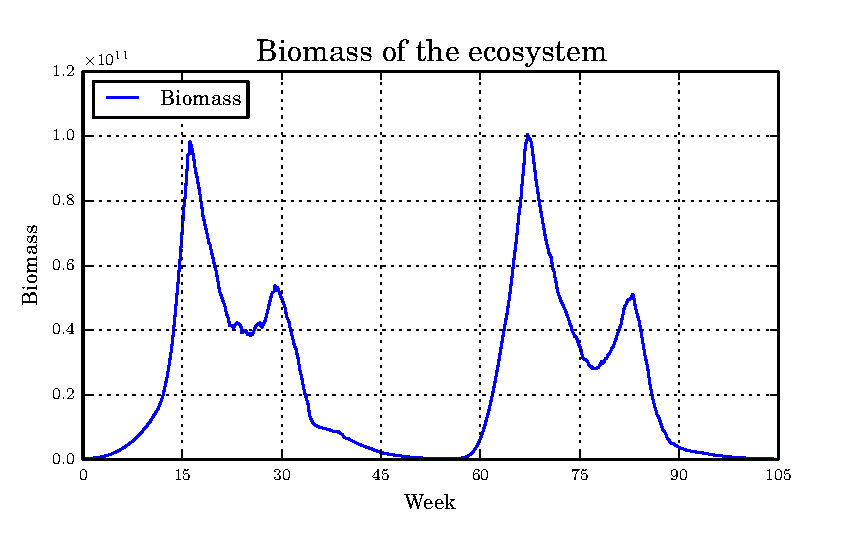
\includegraphics[width=\columnwidth]{graphs/master-bio.eps}
    \caption{Biomass of the ecosystem over time.}
  \end{center}
  \label{fig:master-bio}
\end{figure}

\begin{figure}[ht!]
  \begin{center}
    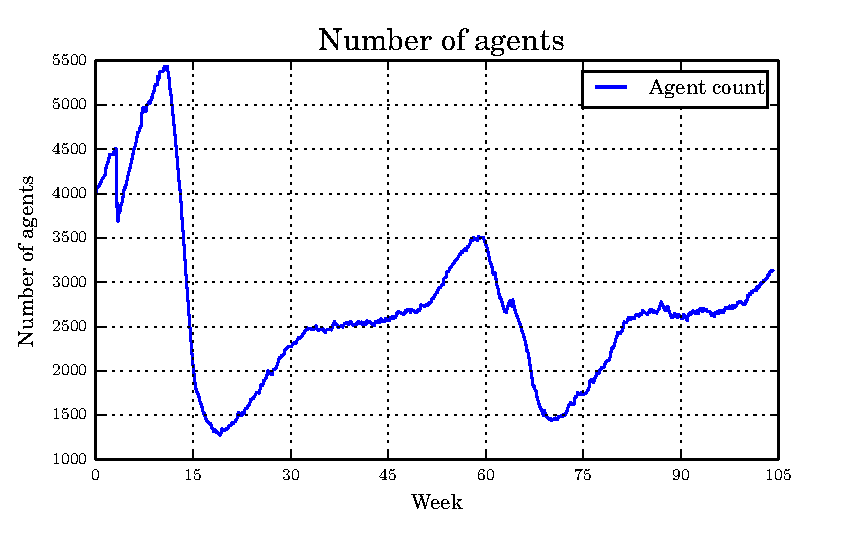
\includegraphics[width=\columnwidth]{graphs/master-ag.eps}
    \caption{Number of agents in simulation over time.}
  \end{center}
  \label{fig:master-ag}
\end{figure}

The simulation itself is an update loop with logic for loading the
environment and storing results. As such it can be summarized by
Listing \ref{list:vew-main-loop}

\begin{lstlisting}[
    caption=Main loop of Simple LERM Model,
    label=list:vew-main-loop,
    language=c,
]
for (t = 0; t < 35040; t++) {
  readPhysics();
  mixChemistry();
  updateAgents();
  updateChemistry();
  particleManagement();
}
\end{lstlisting}

Since our target software has fundamentally different environment management
and initialisation the attention is focused on \lstinline{updateAgents()}
function. That is the place where the embedded Python will get executed
and it contributes bulk of the execution time. Changes to other parts
of the code will be carried out only to allow reliable parallelisation
and correctness of results in multithreaded execution model.

Python is a significantly higher level language than C. Apart from making
the code threadable, the single thread performance should not be sacrificed.
Hence, we begin by benchmarking this implementation and will treat it as
our baseline for performance comparison.

\begin{figure}[ht!]
  \begin{center}
    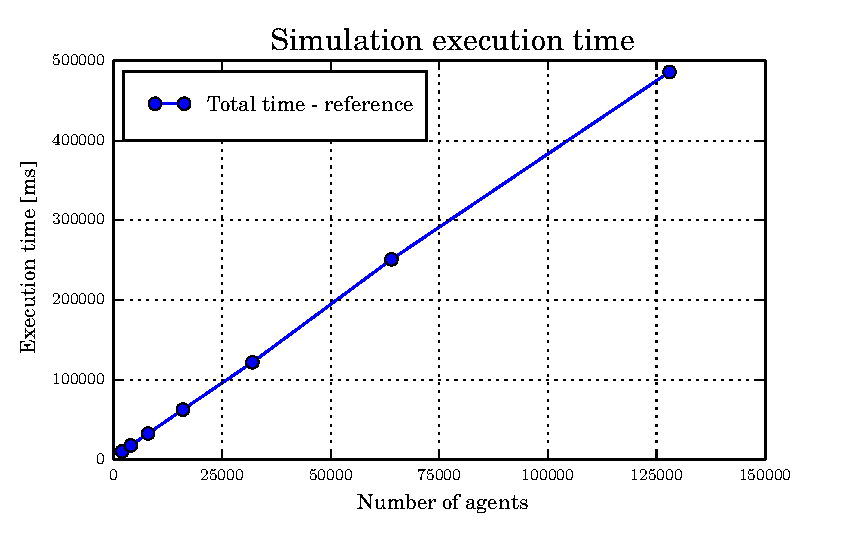
\includegraphics[width=\columnwidth]{graphs/master-perf.eps}
    \caption{Total execution time of simulation for reference version.}
  \end{center}
  \label{fig:master-perf}
\end{figure}

\missingfigure{INCLUDE TABLE WITH ALL VALUES}

\section{Embedding Python}\label{sec:embed-py}
First step is to perform the embedding of Python. In order to do this the
we let Cython generate appropriate C functions and header file.
Then in turn those functions will include provided agent update code.
Hence, if the agent update code needs to be changed the simulation
code does not have to be recompiled (important requirement if porting
to Fluidity is to be useful). The necessary modifications to the simulation
do not require more than what is shown in \ref{sec:embed-cython}. What is left
is replacing the native C update functions with calls to Python versions
and propagating the return values as to preserve semantics of simulation.

The important part is the glue code that performs data transformation from
C to Python. As memory can be a significant bottleneck and constant copying
data back and forth will degrade performance rapidly care has to be taken
to ensure copy-free data passing. Furthermore since in Python the agent
variables are represented as dictionaries while in C they are simple arrays
a wrapping mechanism has to be provided to ensure consistent semantics of
code. Python represents everything as an object inside the interpreter.
As a result every operator actually calls certain function on object in
question. Fortunately CPython, as C++, allows for operator overloading,
therefore allowing us to create a wrapper for an array that behaves
like dictionary.

\begin{lstlisting}[
    caption=Python wrapper for agent array,
    label=list:array-adapter,
    language=python,
]
cdef object agentNames = {
    "AmmoniumIngested" : 0,
    "Ammonium"         : 1,
    "SizeOld"          : 2,
    "SizeNew"          : 3,
    "Carbon"           : 4,
    "Chlorophyll"      : 5,
    "NitrateIngested"  : 6,
    "Nitrate"          : 7,
    "SilicateIngested" : 8,
    "Silicate"         : 9,
    "ZOld"             : 10,
    "ZNew"             : 11,
    "Stage"            : 12
}

cdef class AgentWrapper:

    cdef float * array

    cdef void setData(self, float* vars):
        self.array = vars

    def __getitem__(self, key):
        return self.array[agentNames[key]]

    def __setitem__(self, key, value):
        self.array[agentNames[key]] = value
\end{lstlisting}

\myparagraph{Cython cdef classes}\label{para:cython-cdef}
Beside supporting built-in Python classes Cython also provides second kind of
class: extension types, sometimes referred to as “cdef classes” due to the
keywords used for their declaration. They serve the purpose of mixing C and
Python semantics. Such classes are restricted compared to Python's due to
necessity of conforming to C standards. As a result they are more
memory efficient and faster than generic Python classes. The main difference
comes from the fact that they use C struct to store fields and methods instead
of Python dict. This enables them to store arbitrary C types without requiring
Python wrapper and accessing fields and methods directly at C level without
Python dictionary lookup.

Generic Python classes can inherit from cdef classes but converse is not possible.
Since Cython requires to know the complete inheritance hierarchy to properly lay
out the C structs, and limits it to single inheritance. Python classes, however,
can inherit from any number of Python classes and extension types both in Cython
and pure Python code.

\missingfigure{GRAPH SHOWING CYTHON CODE PERFORMANCE}

\subsection{Finding Bottlenecks}\label{subsec:python-embed-bottleneck}
From the Figure \ref{fig:cython-perf} we immediately see a steep
degradation in performance that happened when the work had been delegated
to Python. Since the resulting code is still single threaded the GIL is
not an issue. What is happening though is change in operation semantics
(Python doesn't have types, hence cannot generate optimised code for primitive types)
and memory accesses (array to dictionary).

To fully understand the extent to which those two factors impacted performance
VTune has been used for analysis.

\missingfigure{VTune output for embedded python}

From output of VTune shown in Figure \ref{fig:cython-vtune} we immediately realise
that due to dynamic nature of Python we have limited insight into actual bottlenecks,
however, it is clear that the the agent update code should be investigated further.

Since the agent code is imported via \lstinline{import diatom} the whole of its body
is managed by Python interpreter. If we compile it as an extension statically
we will be able to investigate parts of it further. That is where Cython helps
us further. Being targeted as easy way to create Python modules the changes necessary
are minimal - adding only another source file to distutils setup script.

\section{Typing update code}\label{sec:embed-py-type}
The difference Cython makes to Python is that it introduces typing in order to generate
efficient code. With agent update code being a pure Python implementation there is
potential for performance improvement without changing the function definitions
and the arguments passed. Section \ref{subsec:cython} shows that fully annotated
code can be significantly faster, however, there types are specified for every
variable present. We will limit the typing to just the code within the agent update.
This task is simplified by the fact that all of the computation inside the update
code are performed on floating point numbers. Hence, for any variable defined we
only have one choice for its type.

\missingfigure{GRAPH SHOWING TYPED CYTHON CODE PERFORMANCE}

Figure \ref{fig:cython-typed-perf} shows that the execution time improved by 60\%.
While the pay-off for fairly simple modification is significant it is not enough
to reach C implementation levels. The code remains more than 20 times slower.
We can conclude that Python semantics impose significant overhead.
For the profiler to be able to analyse the update code directly we can use Cython
C semantics and define functions as \lstinline{cdef} instead of \lstinline{def}.
It effectively means that the function is a pure C function and should be called
as such. \lstinline{cdef} functions cannot be called from Python code.
Cython also provides third keyword for defining functions - \lstinline{cpdef}
which creates both C and Python versions of a function making it accessible in both
languages.

\myparagraph{Interpreted languages}\label{para:interpret-lang}
CPython implements an interpreter for Python language. As such it does not provide
any code generation techniques. With few exceptions interpreted languages do not
generate machine code but operate on internal state which represents the program.
Then it's the role of the interpreter to translate the operations into actions
that are executed by the machine. What this entails is that there is an
abstraction layer between the language and underlying architecture. This
approach provides great deal of flexibility and expressiveness since operations
can be expressed in higher level language than assembly. In case of CPython it
is C which already is a significant improvement over assembly. On the other hand
the effect is that the program cannot be directly tuned for performance. Since
the interpreter mediates the operations between the machine and our code care
has to be taken to produce code that will perform well. Even if the internals
of the interpreter are heavily fine tuned, as it is the case with CPython, the
overhead of function call compared to few assembly instructions is not unnoticeable.
Interpreted languages are often combined with dynamic typing to speed up development.
When writing Python code the programmer does not have to consider types,
array boundaries, memory layout and management. All in all the user can focus
on writing what he wants to achieve and not how to achieve it. However, without
mentioned details and with liberal language semantics the interpreter cannot
produce efficient code. This is the trade off of dynamic typing. PyPy is a
project which aims to recover some of the performance lost due to CPython
interpreter via JIT compiler. From other languages like Java, and to lesser
extent JavaScrip, we can see that JIT equipped interpreters can achieve performance
as good as statically compiled code. Technically there is no reason why Python
should be slower than JavaScript which is the case currently.

\missingfigure{table showing execution time breakdown for cython cdef version}
\todo{Elaborate on numerous python api calls}

\section{Avoiding GIL}\label{sec:embed-c++}
Having in mind the profiling results from previous section we realise that
it's CPython implementation that is slow compared to C. The abstracted numerical
operations, memory management and dictionary references are extremely costly
when compared to machine instructions. To achieve further performance
improvements we need to address the issue of Python runtime dependency.
While it is essential to remove single threaded performance bottlenecks there is
also a more important goal to achieve - enabling multithreaded execution. This
in turn means that we have to find a way to produce GIL free code for the
agent update.

Cython provides useful addition to function definitions \lstinline{nogil} which
states that the function is safe to be executed with GIL released, furthermore
it provides simple checks to ensure that said code is actually GIL free. Since
we have already typed all of the variables defined inside update functions we
have to focus on typing arguments and return values. Agent update code uses
dictionary to define agent parameters. Those define environment constants that
are used for computation when advancing agents to next time step. In principle
there can be more than one parameter set for given agent update code to provide
intra-species variability. Furthermore the agent state and current environment
variables are passed as a dictionary accessible array as outlined in Listing
\ref{list:array-adapter}. The biggest issue we are facing when substituting
dictionaries for something faster is that we do not want to rewrite the whole
agent code since the solution has to be adaptable to arbitrary code provided
by the user. Furthermore C does not provide syntax for dictionaries, hence
with C as a target language there is only one alternative - arrays. However,
Cython can not only target C as a target language but also C++. One of the
features of C++ programming language is operator overloading. It provides
similar capabilities as Python overloading therefore we could substitute Python
dictionaries with optimised C++ implementation. What we want to achieve is a
configurable class with behaviour similar to wrapper presented in Listing
\ref{list:array-adapter}.

\begin{lstlisting}[
    caption=C++ array wrapper,
    label=list:array-adapter-c++,
    language=c++,
]
#include <unordered_map>

template<typename K, typename V>
class ArrayMap {
    private:
        V * dataArray;
        std::unordered_map<K, size_t> dataMap;

    public:
        ...
        void setData(V *);
        void setMapper(std::unordered_map<K, size_t>&);
        V& operator[](const K&);
};

template<typename K, typename V>
V& ArrayMap<K, V>::operator[](const K& key) {
    return this->dataArray[this->dataMap[key]];
};
\end{lstlisting}

Listing \ref{list:array-adapter-c++} shows how such wrapper can be created
(details omitted for brevity). Effectively we create \lstinline{std::unordered_map<K, V>}
with a caveat that the underlying data is stored in a array that we control
instead of the map implementation. We can use this class to pass all of the
dictionaries (agent data, environment variables, environment constants) to
the agent update code. For a long time C++ did not provide built in hash map
implementation. When we look at the documentation of \lstinline{std::map<K, V>}
we will notice that it is actually a red black tree. While in most cases
the difference might not be noticeable - especially if the code performs
many writes to the map. Only C++11 standard provided \lstinline{std::unordered_map<K, V>}
which is implemented as an actual map with $O(1)$ lookup. Given our use case
where the map is only written to once - at creation time - and then only
read from to provide index values to array the \lstinline{std::unordered_map} is
a better solution. It should be noted that performance difference is not large
since our maps are no more than 30 elements in size.

Equipped with C++ version of agent wrapper we only have small changes left.
To avoid any implicit type conversion we need to provide full type definition
for function prototypes. Therefore we change Listing \ref{list:agent-update-fn-proto}
to Listing \ref{list:agent-update-fn-proto-full}. Such replacements can in principle be
automated, however, we will see how to make the type signature simpler in later sections
thus removing long type declarations.

\begin{lstlisting}[
    caption=Agent update function prototype,
    label=list:agent-update-fn-proto,
    language=python,
]
def update_Living_Diatom(vars, env):
\end{lstlisting}

\begin{lstlisting}[
    caption=Agent update function prototype,
    label=list:agent-update-fn-proto-full,
    language=python,
]
cdef void update_Living_Diatom(ArrayMap[string, float]& vars, ArrayMap[string, float]& env, float * rel) nogil
\end{lstlisting}

\missingfigure{GRAPH SHOWING GIL FREE CODE PERFORMANCE}

\subsection{Scalability}\label{subsec:embed-c++-scala}
\missingfigure{GRAPH SHOWING GIL FREE CODE SCALABILITY - UP TO 4 threads}


\subsection{Further Optimisations}\label{subsec:further-opt}
\missingfigure{table showing execution time breakdown for c++ version}

\section{Removing hash maps}\label{sec:remove-dict}
\missingfigure{GRAPH SHOWING ARRAY TYPED VERSION}
\missingfigure{TABLE of results from profiler}

\subsection{Scalability}\label{subsec:embed-array-scala}
\missingfigure{GRAPH SHOWING GIL FREE CODE SCALABILITY - UP TO 4 threads}

\section{Summary}\label{sec:simple-lerm-summ}
\missingfigure{GRAPH SHOWING ALL CODE VERSION FOR 1 THREAD}


\chapter{Fluidity Simple LERM Model}\label{ch:thread-fluid}

\section{Implementation differences}\label{sec:impl-diff}

\section{Compiling agent code}\label{sec:compl-agent-code}

\chapter{Evaluation}\label{ch:evaluation}

\section{Initial vs Target performance}\label{sec:init-vs-target}

\section{Parallel execution via C++}\label{sec:para-c++}

\section{Using arrays}\label{sec:array-use}

\section{Scalability}\label{sec:scalability}

\section{Model Correctness}\label{sec:model-correct}

\section{Fluidity}\label{sec:fluid-appcl}

\chapter{Conclusion}\label{ch:concl}

\section{Summary}\label{sec:summary}

\section{Related Work}\label{sec:related}

\subsection{PyPy Software Transactional Memory}\label{subsec:pypy-stm}
\subsection{PyParallel}\label{subsec:pyparallel}
\subsection{Jython and IronPython}\label{subsec:other-python-impl}

\section{Future Work}\label{sec:future}

% To add something to the bibliography, look for the "import into BibTex" thingy on google scholar, and add the stuff into refs.bib.
\bibliographystyle{plain} \bibliography{References}

\end{document}
\end{figure}
